\documentclass[11pt]{article}
\usepackage{url,amsmath,bm,graphicx,listings,caption,subcaption}
\usepackage[style=numeric,backend=bibtex]{biblatex}
\title{E4301 Project: Adaptive Mesh Refinement Regridding Intervals}
\author{Andrew Kaluzny (akk2141)}
\date{December 23, 2014}

\addbibresource{bibliography.bib}

\begin{document}
\maketitle

\section*{Introduction}
Adaptive mesh refinement (AMR) allows for the efficient handling of problems
that involve multiple scales by increasing mesh resolution only when and
where it is needed. This provides the potential for substantial performance
gains, as a coarser mesh can be used for the parts of the problem where it
is appropriate. These performance gains offer the possibility not just of
more convenient modelling, or higher accuracy solutions in the same time
frame, but also opening new uses for numerical models (such as quickly
running a model over a distribution of initial parameters that capture
uncertainty in their values, and using the outcome to find the uncertainty
in the results).

AMR brings a new set of parameters to a numerical model, including how 
regions are chosen for refinement, how frequently refinement occurs,
and how refined regions interact with each other as well as coarser meshes.
Among these parameters, there exists a relationship between the 
time between refining the mesh
and the regions chosen for refinement; the longer the interval between
refinements, the larger the refined regions must be to ensure that any
interesting feature that needs the higher resolution doesn't move somewhere
else before the next refinement step is able to reposition the finer mesh
appropriately. It is this relationship I am interesting in exploring, and
its effect on the run time of the model as a whole. If the refinement process
is particularly costly, increasing the time between those steps is advantageous,
but it is balanced by the need to increase the size of the refined regions.

To explore this trade-off, I used the Clawpack software,
and its AMR implementation, AMRClaw (see \cite{clawpack}), 
to look at two sample problems and how
their solutions react to changing the time between refinement and the buffer
added around refined regions to counteract that time.

\section*{Adaptive Mesh Refinement in Clawpack}
Clawpack is a suite of software tools for solving hyperbolic systems of
PDEs using finite volume methods. The use of finite volume methods make it
particularly suited to systems of conservation laws, for example modelling storm surges and tsunamis (where the differing scales 
between the expanse of the ocean and details of harbors make AMR a useful
tool).

AMRClaw is Clawpack's AMR implementation (and its operation is described
in more detail in \cite{BergerLeVeque98}). The mesh takes the form of a 
rectilinear grid. Grid cells are flagged for refinement based on some criteria
exceeding a threshold (in this case the maximum of the differences between
neighbouring cells), and then clustered into rectangular patches that each
act as a new, finer grid. A refinement also occurs in the time step, to
ensure the CFL condition is still met, and thus several time steps occur
on the finer grids for each step on the coarser grid. Boundary conditions
are implemented using ``ghost'' cells which get their values either from
the boundary conditions of the whole problem, from neighbouring refined grids, 
or by interpolating from coarser grids.

There are two runtime parameters provided by AMRClaw for specifying the
interval between regridding (as the number of steps to take on each
level before recomputing the refinement criteria and redrawing the patches)
and a buffer width (as the number of cells in each direction around the
flagged cells which also need to be included for refinement).

\section*{Running Parameter Sweeps and Gathering Data}
To keep the scale of my project reasonable, I decided to focus on two examples
provided with the AMRClaw software: the advection of a square region on a domain
with periodic boundary conditions, and a gas dynamics problem using the Euler
equations for non-viscous, adiabatic flow on a domain with four quadrants of
differing density. The advection problem offers a simple and easily understandable
problem for investigation; the expected behaviour of the solution is clear and
the regions of interest for refinement are intuitively the boundary of the square.
The Euler gas problem offers a more complex, physical problem that hopefully has
features that make it closer to the kind of problem one would want to solve
in practice.

Though the advection problem has an easy analytical solution, the gas problem
does not. Thus for computing errors I used a run of the problem on which a 
single grid at the finest level was used as an approximate ``true'' solution.
This choice is particularly suited to AMR, where the goal is effectively to
get a solution like the one using a fine grid everywhere, without having 
actually done so. Comparing solutions when differing grids are involved is not
as straightforward as when a single uniform grid is involved, but AMRClaw 
allows one to specify ``gauge'' points where the solution will be logged
independent of the actual grid, interpolating as necessary.
A relative $L_1$ error was thus computed by sampling from a series of gauge
points in both time and space (as a compromise between observing a few points
closely over time or looking at the whole solution at only one time).

To run the problems over a series of parameters, I created a script
\texttt{run\_param\_sweep.py}\footnote{Professor Mandli directed me to some
existing scripts for running parameter sweeps, but I was having trouble
adapting it to my specific case. I gambled that with the time available to me
it would be easier to create scripts for exactly what I needed than trying to
reverse engineer a more complex, fully featured system to figure out how it
worked.} to copy a base version of the problem directory repeatedly,
modifying the \texttt{setrun.py} in each copy to have the necessary 
regridding parameters. A second script, \texttt{parse\_runs.py}, provides
functions to read the output files, aggregate the data, and plot the
results.\footnote{The images of the solutions themselves and the placement of 
various grids, however, come from the tools provided by Clawpack. 
I would like to thank Professor Mandli for providing code for visualizing
the values of the refinement criteria and their location relative to the
various grids.}

\section*{Regridding in a Simple Advection Problem}
In the simple advection example provided in AMRClaw, a square region moves
towards the upper right corner of a square domain (periodic in both the 
x and y directions), returning to its original position at time $t=2$. For a reference
solution, I used a grid with 200 cells on each side and no refinement
(see Figure~\ref{fig:advec_base}). The
AMR solutions all used a grid that started at 50 cells each side, and had
two levels of refinement (by a factor of two each time, for a finest grid
with cells one-fourth the width of the initial cells), making its finest 
cells the same size as those used everywhere in the reference solution.

\begin{figure}[!htb]
\centering
	\begin{subfigure}[b]{0.45\textwidth}
		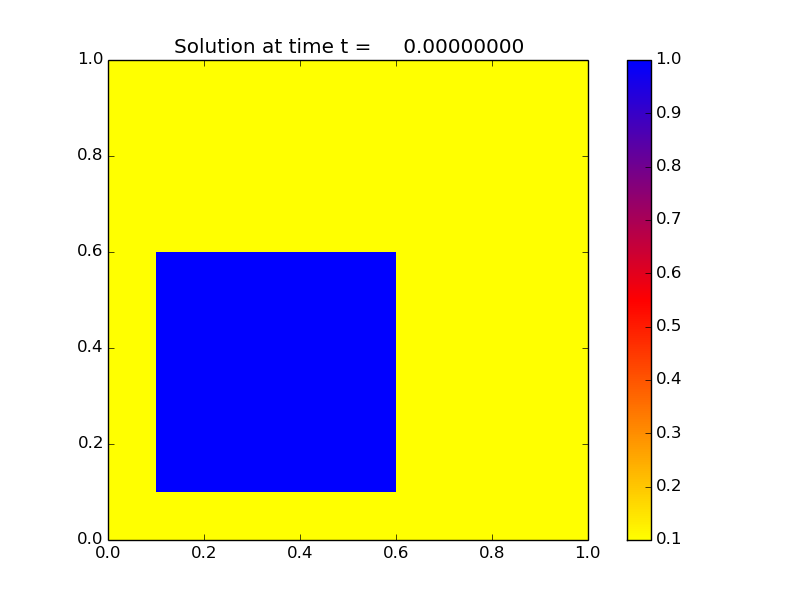
\includegraphics[width=\textwidth]{images/advec_base_t0}
	\end{subfigure}
	\begin{subfigure}[b]{0.45\textwidth}
		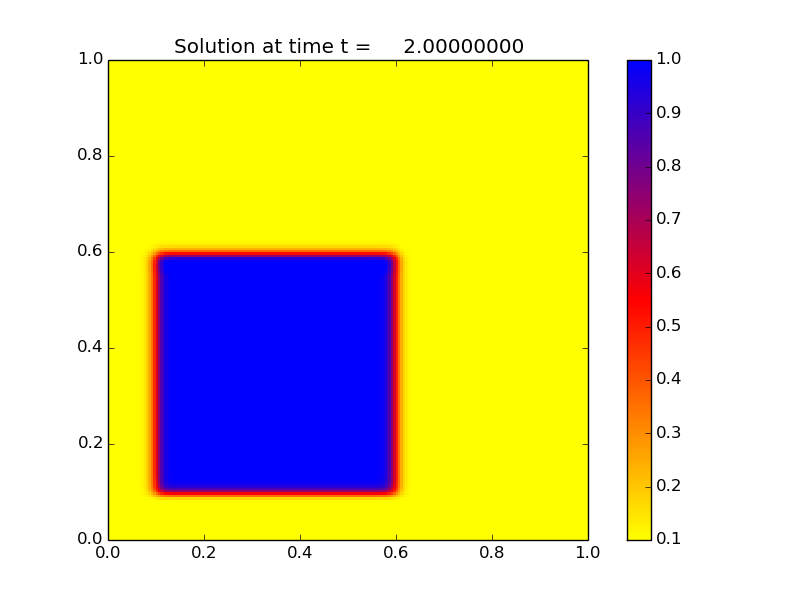
\includegraphics[width=\textwidth]{images/advec_base_t2}
	\end{subfigure}
	\caption{The start and end of the solution to the advection problem
			computed on the finest grid.}
	\label{fig:advec_base}
\end{figure}


First, I wanted to confirm the need to vary the regridding interval and
buffer width in tandem with each other. To do this, I did ten runs of the
AMR setup with buffer width of 1, but with regridding intervals from 1 to
10. We expect the regridding interval cannot exceed the buffer width by
much without causing a non-trivial loss in accuracy. As the CFL condition
constrains waves to moving through roughly one grid cell per time step,
every step between regridding moves any finely resolved feature one
cell closer to escaping a refined area, essentially losing information
to the coarser grid.

The relative $L_1$ error (as compared to the fine grid reference solution)
as a function of the regridding interval can be seen in 
Figure~\ref{fig:err_advec_bad}. As expected, the error increases with the
regridding interval (roughly tripling once the interval reaches 9); the 
relative stability of the error until the interval reaches 4 can be expected
from the ``natural'' buffering produced by aggregating cells flagged for 
refinement into rectilinear patches. 
The plateau that begins to form around an interval of 8 could indicate a limit
to the ``badness'' of letting things escape from finer grids. Once the interval
between regridding steps becomes large enough, most everything of interest
may leave the refined region and become lost in the coarser grids. The point
at which this occurs likely depends on the specifics of the problem, but in
this advection problem, where everything moves at a constant rate and the 
regions of interest are rectilinear and at a fixed angle to the motion of
the square, we might expect a relatively clear and well-defined plateau
as things will move out of the refined regions at a predictable and
unchanging rate.

\begin{figure}[!htb]
\centering
\caption{Relative $L_1$ error for the advection problem, with the buffer
width held constant at 1.}
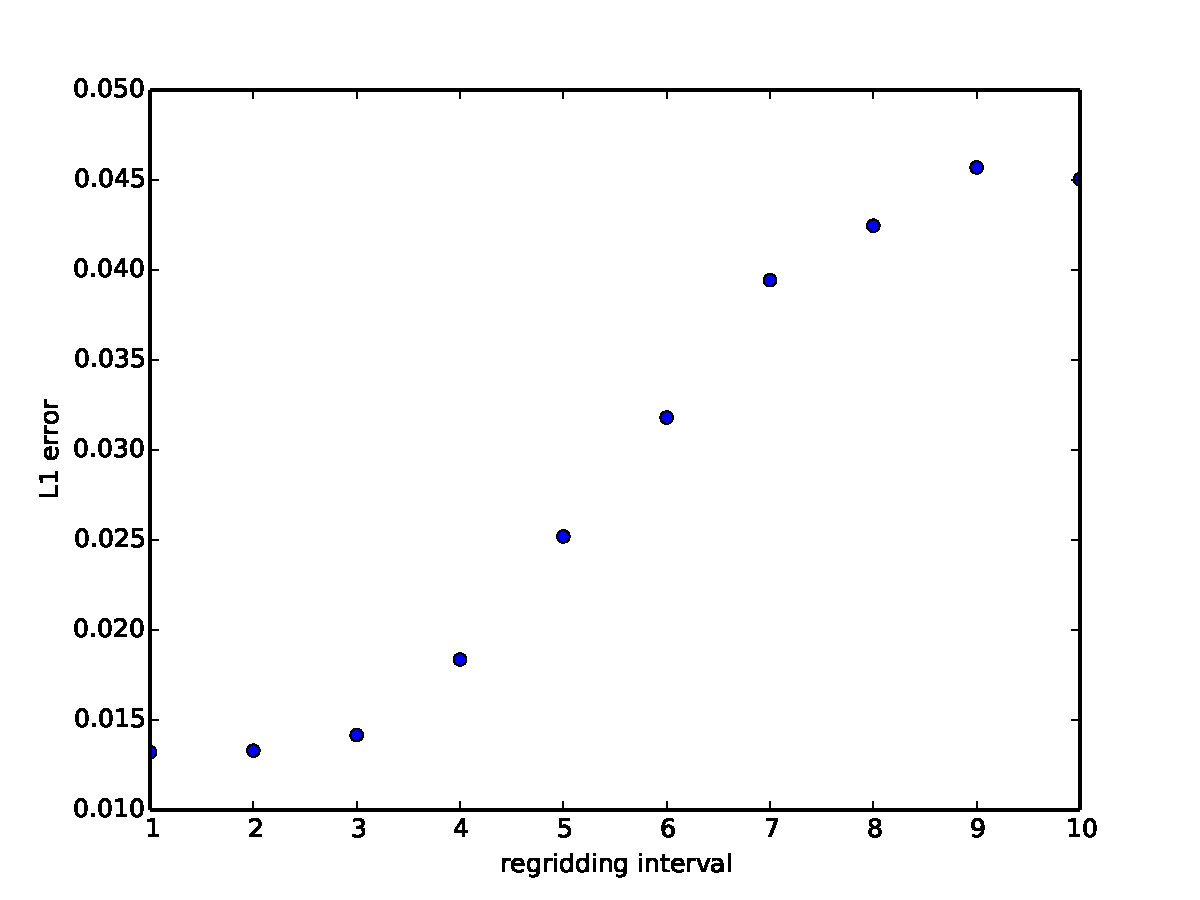
\includegraphics[width=0.85\textwidth]{myclaw/l1_err_advec_bad}
\label{fig:err_advec_bad}
\end{figure}

The running time for these ``bad'' solutions can be seen in 
Figure~\ref{fig:rel_time_advec_bad}. The jump up at interval 2 appears
to be an anomaly, and doesn't match with any change in the number of
cells or the error. Otherwise, the running time is relatively constant,
its peaks might be random variation in the running time, or the interactions
between the decreased time from a larger interval, the slight increase in
level 2 cells, and the slight decrease in level 3 cells as the interval
increases. These trends in the number of cells can be seen in 
Figure~\ref{fig:avg_cells_advec_bad}, and likely arise from the increasing
``badness'' of the solution, which manifest as a more dispersed square,
which covers more area (thus more level 2 cells), but has a more gradual
slope to its edges (thus smaller differences over short distances and
fewer level 3 cells).

\begin{figure}[!htb]
\centering
	\caption{Running time and cell coverage as a function of the regridding
	interval for the advection problem, with buffer width held at 1.}
	\begin{subfigure}[b]{0.65\textwidth}
		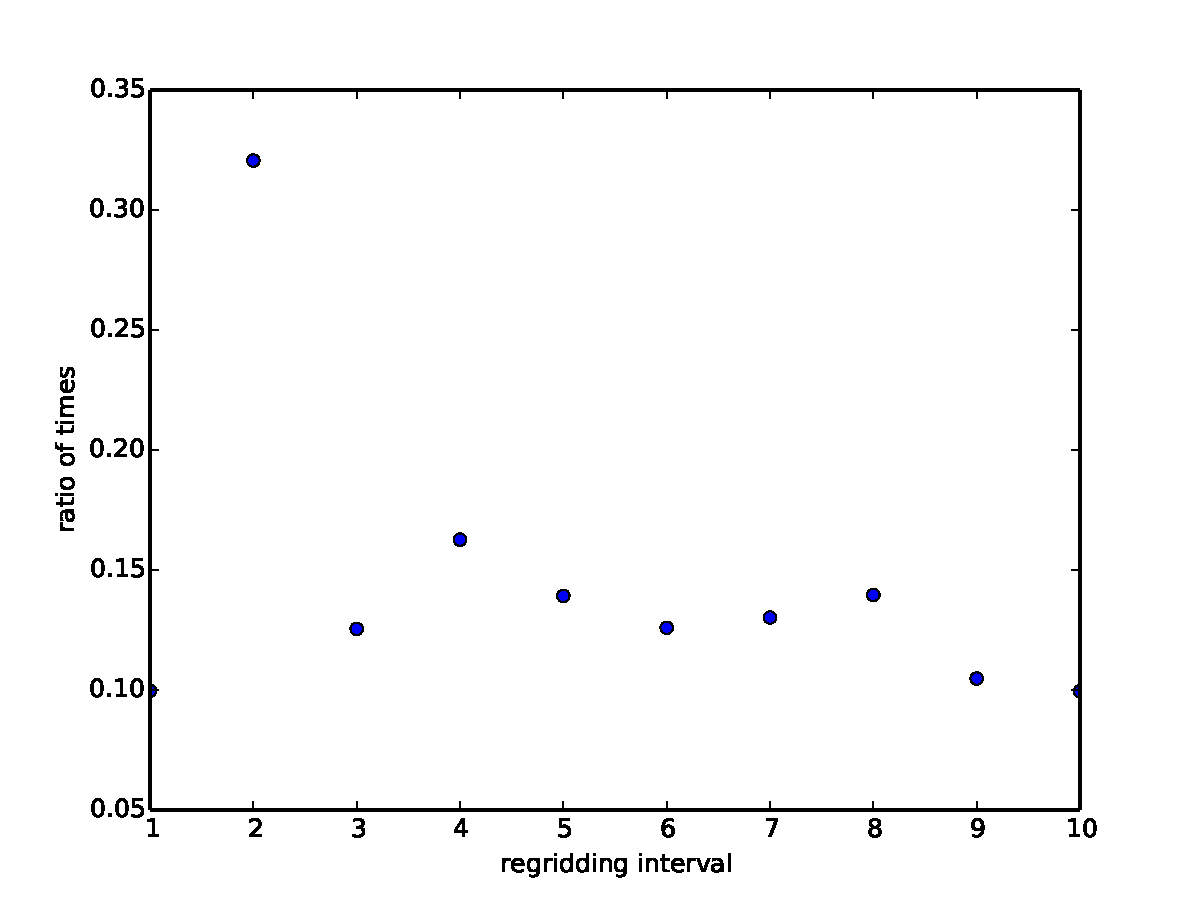
\includegraphics[width=\textwidth]{myclaw/rel_time_advec_bad}
		\caption{Running time (as a fraction of the running time of the 
		reference solution)}
		\label{fig:rel_time_advec_bad}
	\end{subfigure}
	
	\begin{subfigure}[b]{0.65\textwidth}
		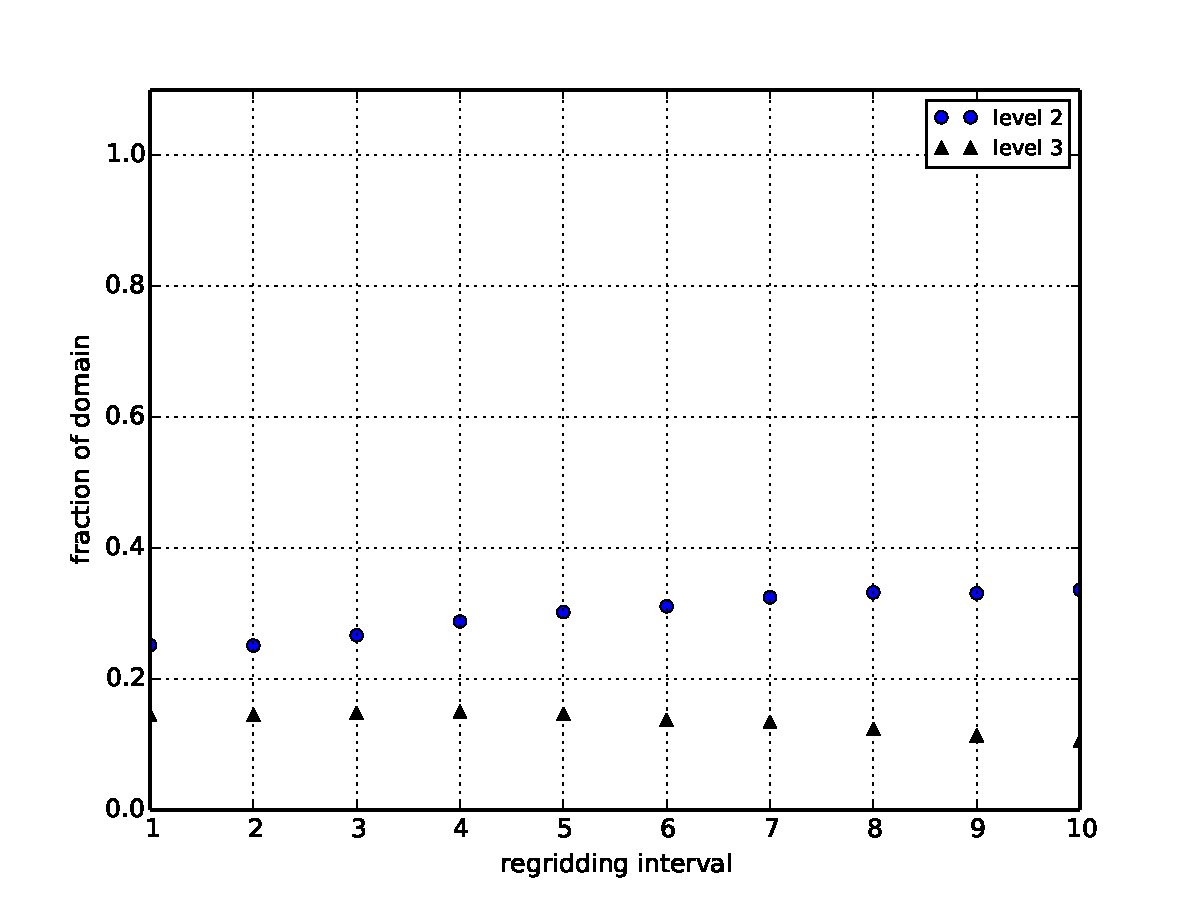
\includegraphics[width=\textwidth]{myclaw/avg_cells_advec_bad}
		\caption{Number of cells on each level (averaged over the whole
		computation) as a fraction of the total domain}
		\label{fig:avg_cells_advec_bad}
	\end{subfigure}
\end{figure}

With the need to keep the regrid interval and buffer width in tandem confirmed,
I did ten runs where the interval and width were equal to each other,
ranging again from 1 to 10. The $L_1$ error as a function of the regrid interval
and buffer width can be seen in Figure~\ref{fig:err_advec}. Here we see the
error decreasing as the interval/buffer increases, which is expected, as the
higher buffer essentially corresponds to more of the problem being solved on
finer grids at any given time. The drop in error is relatively minor compared
to the blow-up of the error when the buffer was fixed, and it plateaus past 
an interval/buffer of 6. This corresponds to when the buffer is large enough
for the second level to encompass essentially the entire domain (see 
Fugure~\ref{fig:avg_cells_advec}).

\begin{figure}[!htb]
\centering
\caption{Relative $L_1$ error for the advection problem, with the number of
buffer cells equal to the regrid interval.}
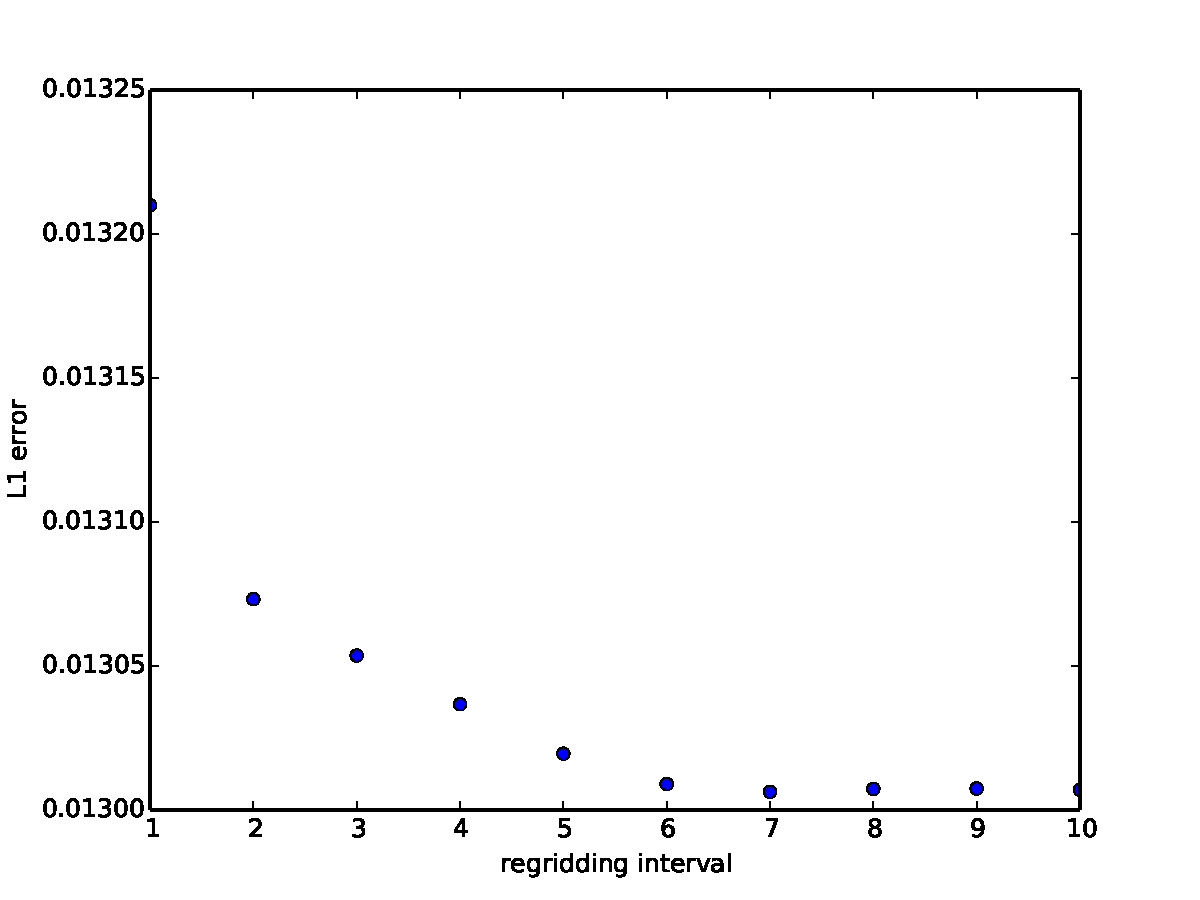
\includegraphics[width=0.85\textwidth]{myclaw/l1_err_advec}
\label{fig:err_advec}
\end{figure}

It should be noted that this error is still relatively large, considering
that with a regrid interval of 10 the problem is being solved on a level 2
grid everywhere, and a level 3 grid (the same resolution as the reference 
solution) over 60\% of the domain (and that that 60\% is focused around
the areas of interest). This may in part be due to the nature of the error
estimate being used, combined with the specifics of the problem. Since the
boundary of the square is ideally a step function, any slight difference
in position or diffusion of the boundary could lead to very large errors,
and since only 25 points are being sampled from, this may not be enough to 
wash out those with the low errors of the vast areas that do agree.

\begin{figure}[!htb]
\centering
\caption{Average number of cells on each level for the
advection problem, with the number of
buffer cells equal to the regrid interval.}
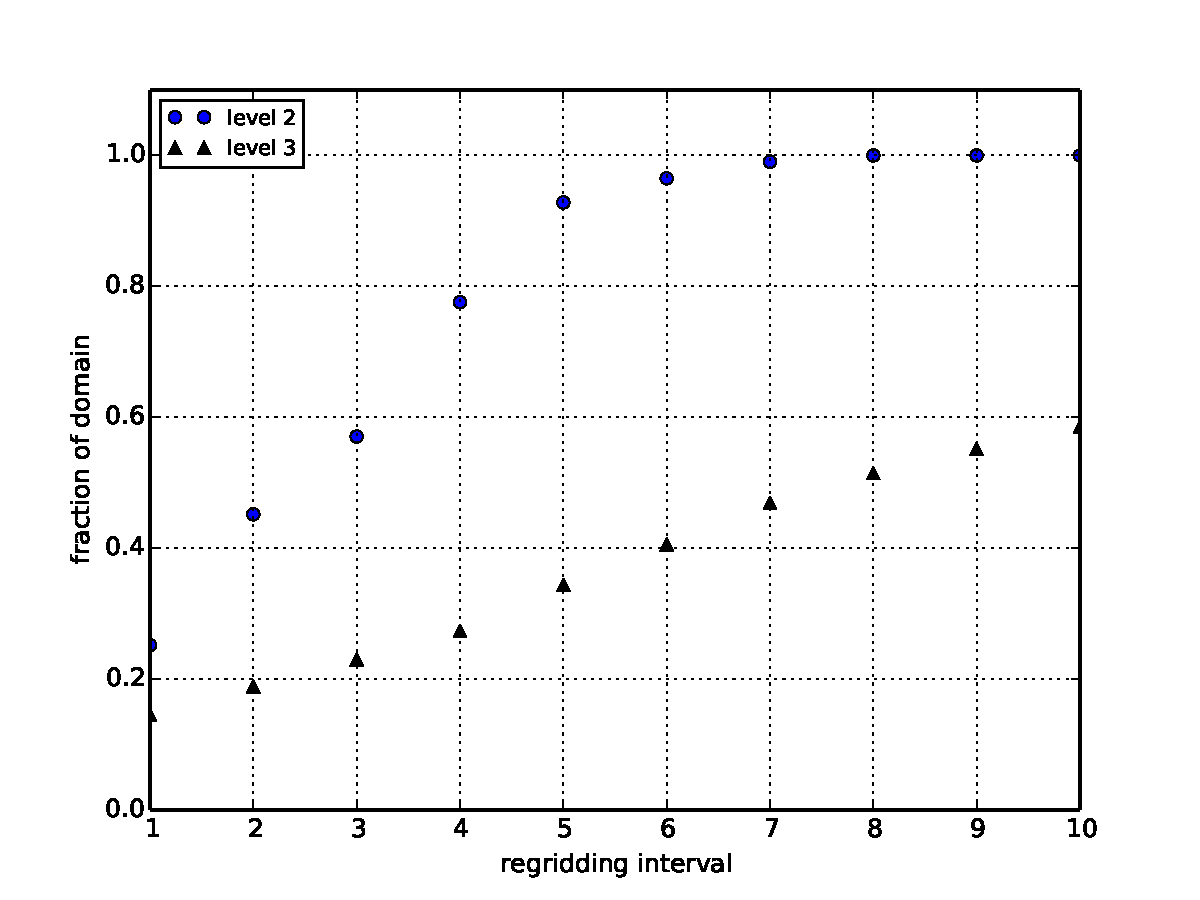
\includegraphics[width=0.85\textwidth]{myclaw/avg_cells_advec}
\label{fig:avg_cells_advec}
\end{figure}

Information on the time taken by each run is in Figure~\ref{fig:time_advec}.
The time is broken down into components: the time spent advancing the
solution on the grids, the time spent regridding, and the time spent updating
grids with information from more refined ones (the total running time is
considered to be the sum of these components, ignoring any io or logging
time). The time spent on the grids is clearly dominant, and as expected
rises as the buffer width increases and more cells exist on each level.
Similarly the general decrease of regridding time is expected as the interval
between regrids increases\footnote{However, the plateau it seems to reach
is less expected. Perhaps as more cells are flagged for inclusion by the 
increasing buffer, the algorithm that clusters them into patches becomes
less efficient.},
and as the number of cells on each level increases,
we expect more time to be taken updating grids.
The increase at an interval/buffer of 3 may be an anomaly (since it does
appear in all three components) or it may be a particularly inefficient
arrangement of flagged cells leading to unnecessarily large grid patches
when combined with the buffer width.

\begin{figure}[!htb]
\centering
\caption{Timing information for runs of the advection problem,
with the number of buffer cells equal to the regrid interval. Note that
at their slowest, the AMR runs take approximately 40\% of the time of the
reference solution.}
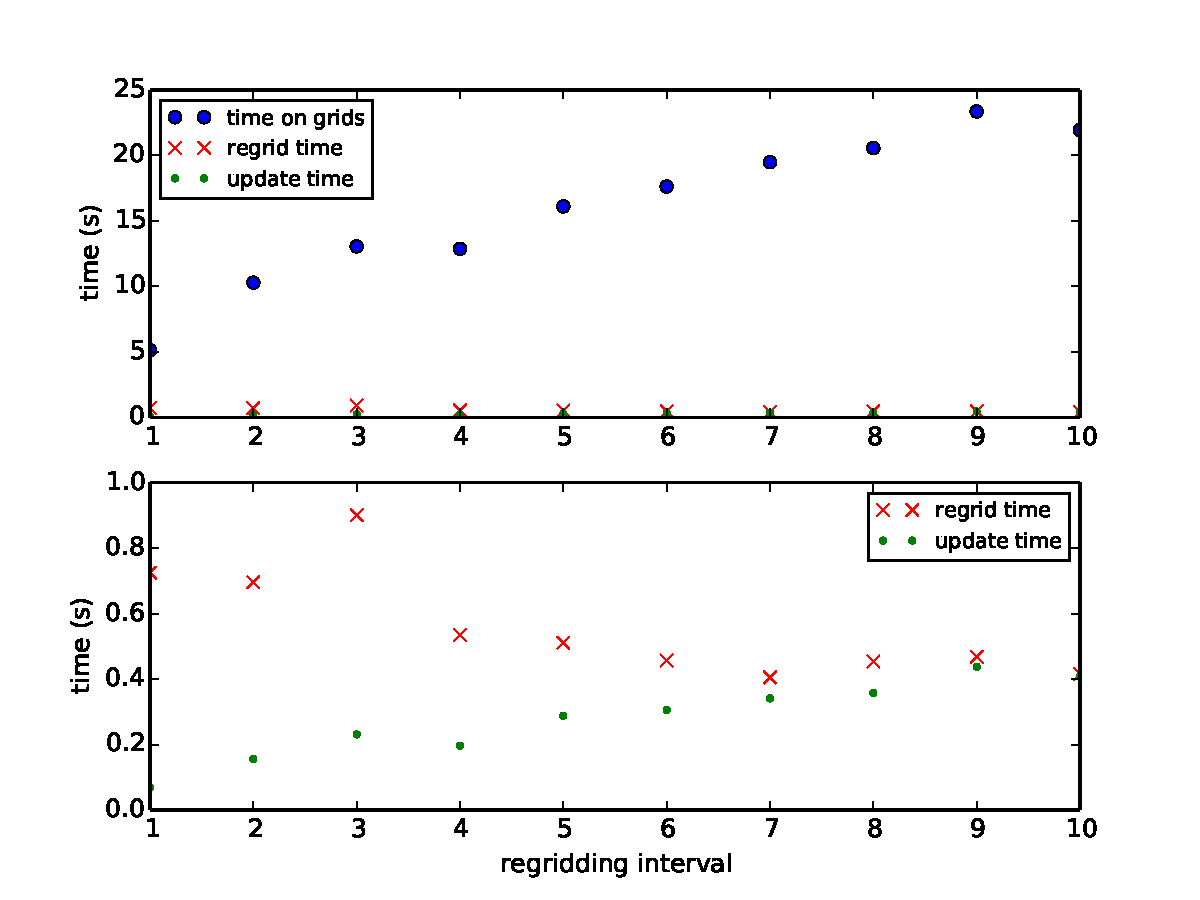
\includegraphics[width=0.85\textwidth]{myclaw/time_advec}
\label{fig:time_advec}
\end{figure}


\section*{Regridding in an Euler Gas Problem}
A similar analysis was then performed for the example Euler gas problem.
The reference problem was run with a 320 by 320 grid; the AMR versions
tarted with a 40 by 40 grid and a total of three levels, refining each 
dimension by a factor of 2 from the first to the second, and by a 
factor of 4 from the second to the third.
Since the problem is more complex and runs on a finer grid, its runs took
much longer and thus runs were only done for even regrid intervals, from
2 to 10.

Just like the advection problem, the Euler problem behaved poorly when the
regrid interval was increased in excess of the buffer width (see
Figure~\ref{fig:err_euler_bad}).\footnote{The data for these ``bad'' runs
ends at an interval of 8, as I was having a problem parsing the output
for the run at 10, and was unable to diagnose the problem in time.} In
this case, the increasing error manifested as more than just a blurring
of the solution, but also in more qualitative discrepancies. 
Figure~\ref{fig:euler_bad_soln} shows a comparison between the reference
solution and one where the regrid interval was allowed to exceed the buffer.
Asymmetries arise in the ``bad'' solution, with the center appearing
swirled or twisted relative to the reference.\footnote{Presumably these
asymmetries come from asymmetries in the clustered grid patches produced
in the regridding step, as that clustering is not constrained to be
necessarily balanced or symmetric. Some parts of the solution are thus
refined over a wide enough area to track fine features for a longer time,
while in other areas those features move out of the refined patch more
readily.}
The ``bad'' solution also
has far more substantial curling structures on some of the boundaries
between densities. I am not sure whether these curled features are
supposed to be present or not, but the asymmetry is concerning, and there
is clearly a danger in increasing the regridding interval beyond just 
coarsening or blurring the solution.

\begin{figure}[!htb]
\centering
\caption{Relative $L_1$ error for the Euler problem, with the buffer
width held constant at 1.}
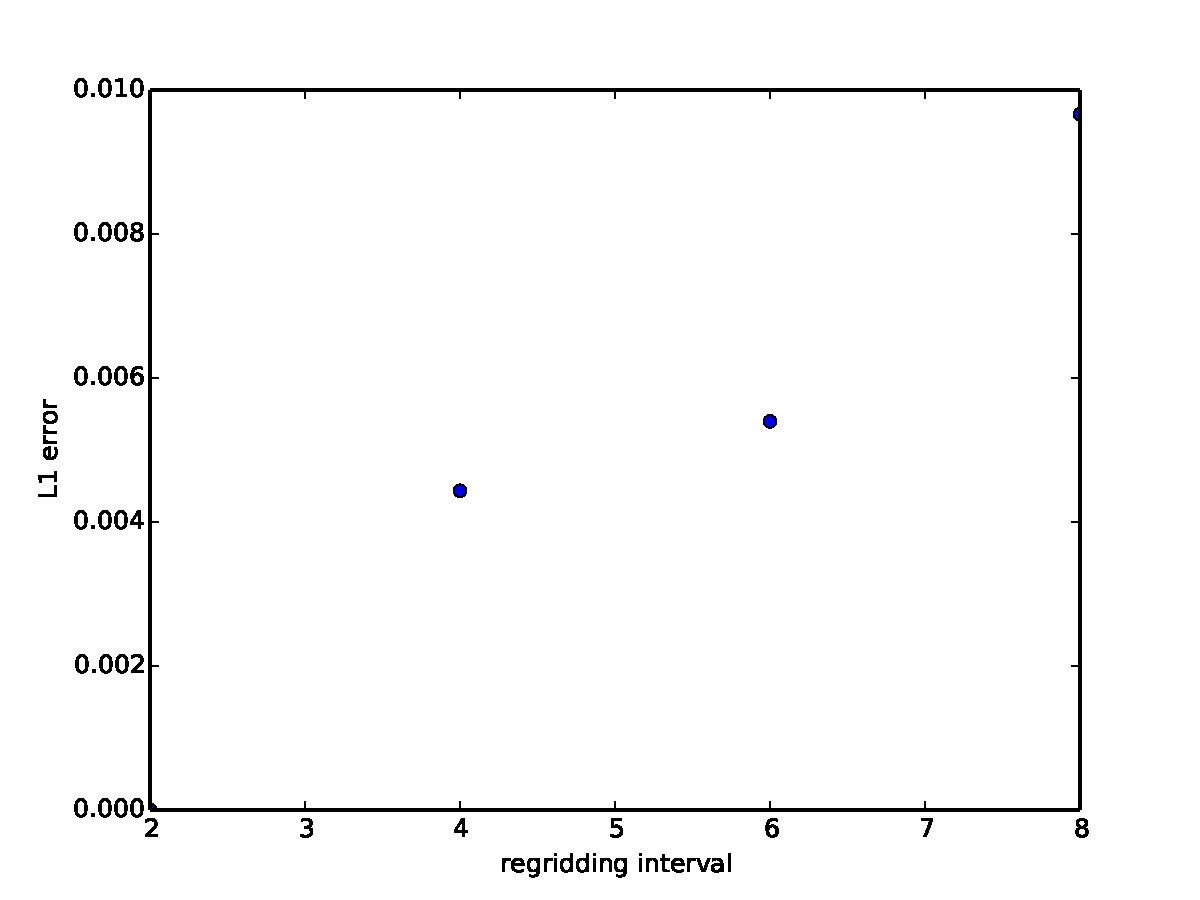
\includegraphics[width=0.75\textwidth]{myclaw/l1_err_euler_bad}
\label{fig:err_euler_bad}
\end{figure}

\begin{figure}[!htb]
\centering
	\begin{subfigure}[b]{0.75\textwidth}
		\caption{Reference solution}
		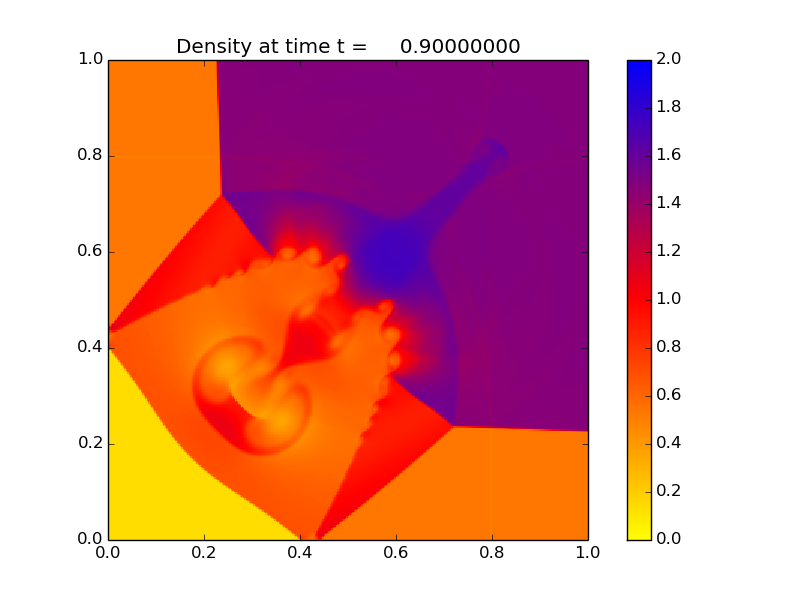
\includegraphics[width=\textwidth]{images/euler_base_t9}
	\end{subfigure}
	
	\begin{subfigure}[b]{0.75\textwidth}
		\caption{Bad solution}
		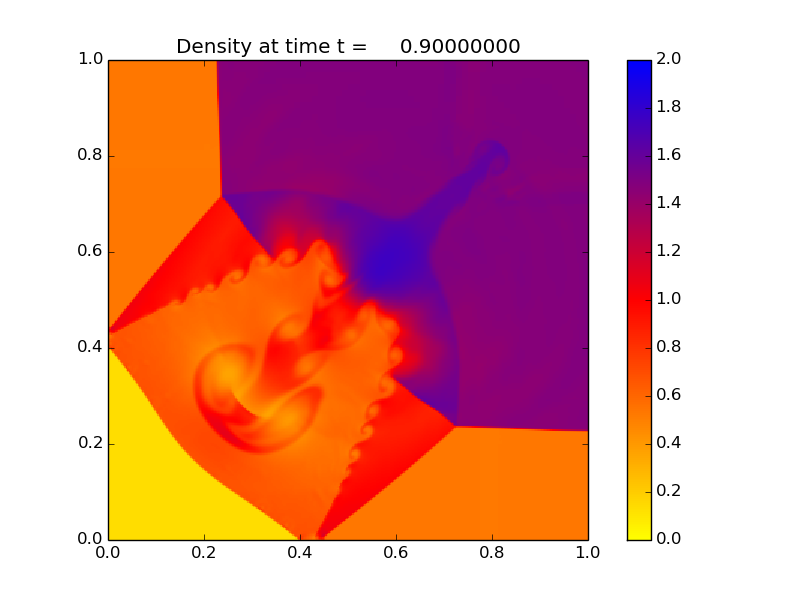
\includegraphics[width=\textwidth]{images/euler_bad_t9}
	\end{subfigure}
	\caption{A comparison between the reference solution, and a ``bad''
	solution (with a regrid interval of 8), showing qualitative distortions.}
	\label{fig:euler_bad_soln}
\end{figure}

When keeping the buffer width tied to the regrid interval, the results
from the Euler problem were again similar to the advection results above.
The $L_1$ error drops then seems to roughly plateau, though again the
drop is not too substantial (see Figure~\ref{fig:err_euler}). Timing is
even more dominated by the time spent on the grids (likely due to the more
complex nature of computing the flux between cells, compared to the relatively
trivial advection problem), but otherwise the overall direction and 
potential to plateau for each
quantity is the same as the interval/buffer increases (see 
Figure~\ref{fig:time_euler}).

\begin{figure}[!htb]
\centering
\caption{Relative $L_1$ error for the Euler problem, with the number of
buffer cells equal to the regrid interval.}
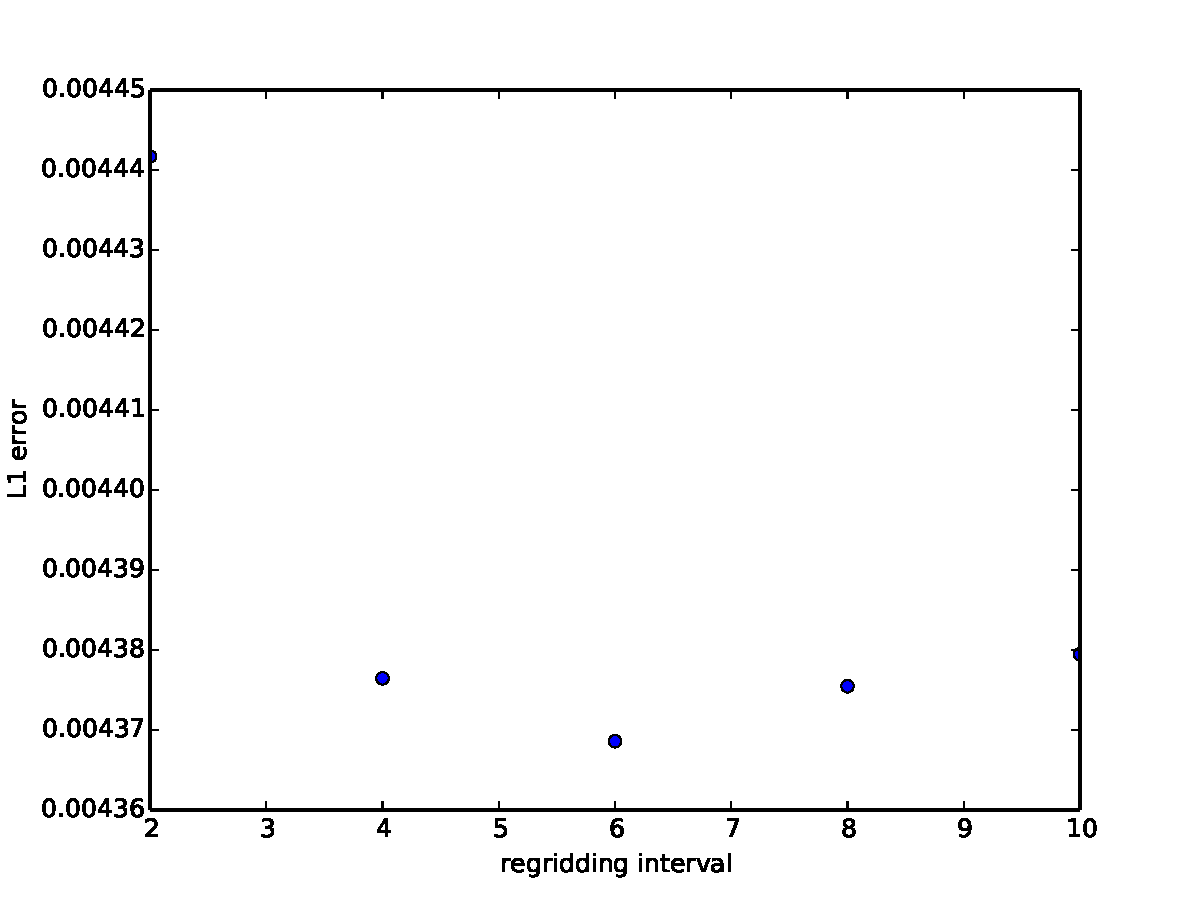
\includegraphics[width=0.85\textwidth]{myclaw/l1_err_euler}
\label{fig:err_euler}
\end{figure}

\begin{figure}[!htb]
\centering
\caption{Timing information for runs of the Euler problem, with the
with the number of buffer cells equal to the regrid interval. Note that
at their slowest, the AMR runs take approximately 75\% of the time of the
reference solution.}
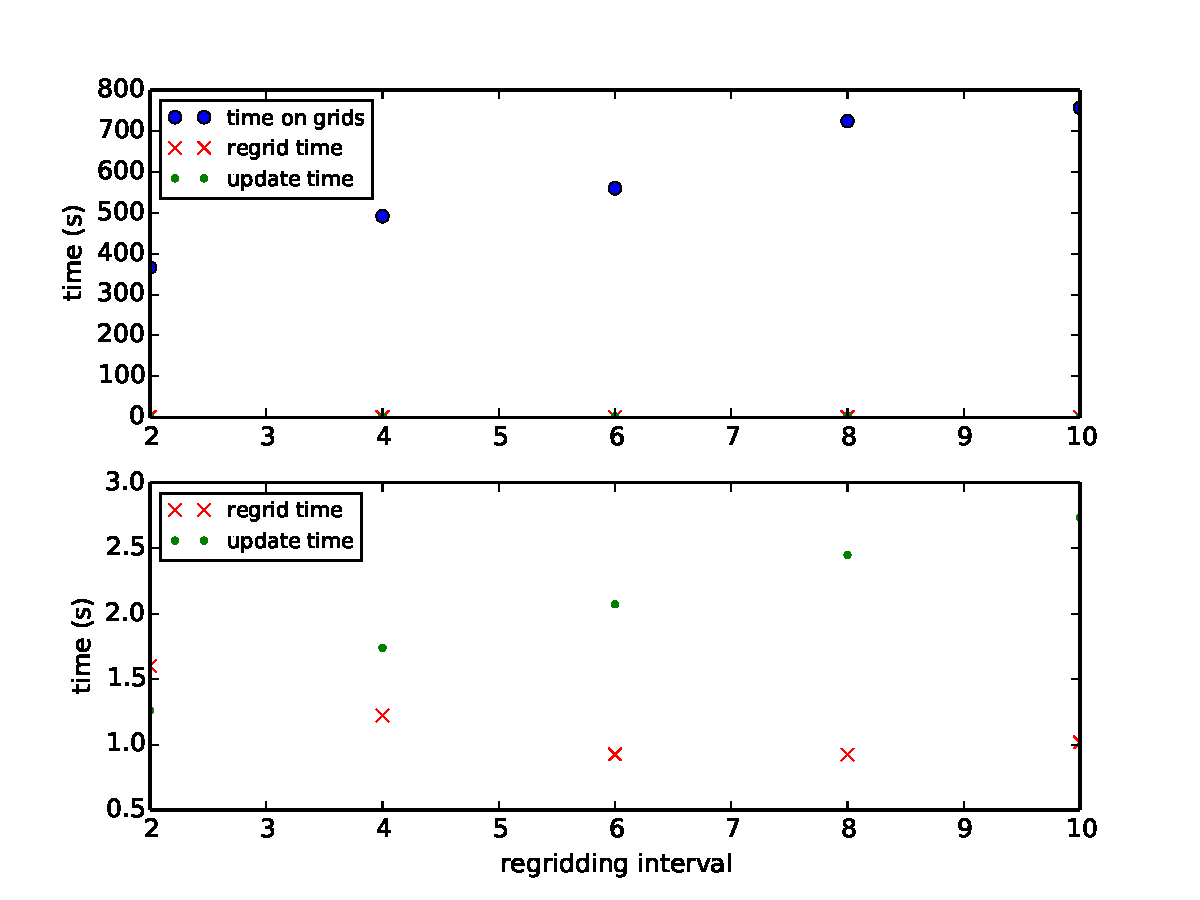
\includegraphics[width=0.85\textwidth]{myclaw/time_euler}
\label{fig:time_euler}
\end{figure}

Behavior of the average number of grid cells on each level was overall
similar to the advection problem--level 2 cells eventually cover the whole grid,
and the number of level 3 cells increases steadily (see 
Figure~\ref{fig:avg_cells_euler}). However, it should be noted that the number of
cells on each level over time in a single run was different between the advection
and Euler problems. In the advection problem, the area of interest remains 
relatively constant in size and shape, but in the Euler problem that area
grows substantially. Thus the number of cells on all levels grows to consume
the whole domain of the Euler problem even in the case where the interval/buffer
is only 2. Thus while the length of the time domain would likely not change
much in the case of the advection problem in terms of effect of increasing
the interval/buffer value, it could have a non-trivial impact for the Euler
problem. (See Figure~\ref{fig:cells_over_time} for a comparison of the
two problems, and the impact of interval/buffer size on the Euler problem.)

\begin{figure}[!htb]
\centering
\caption{Average number of cells on each level for the
Euler problem, with the number of
buffer cells equal to the regrid interval.}
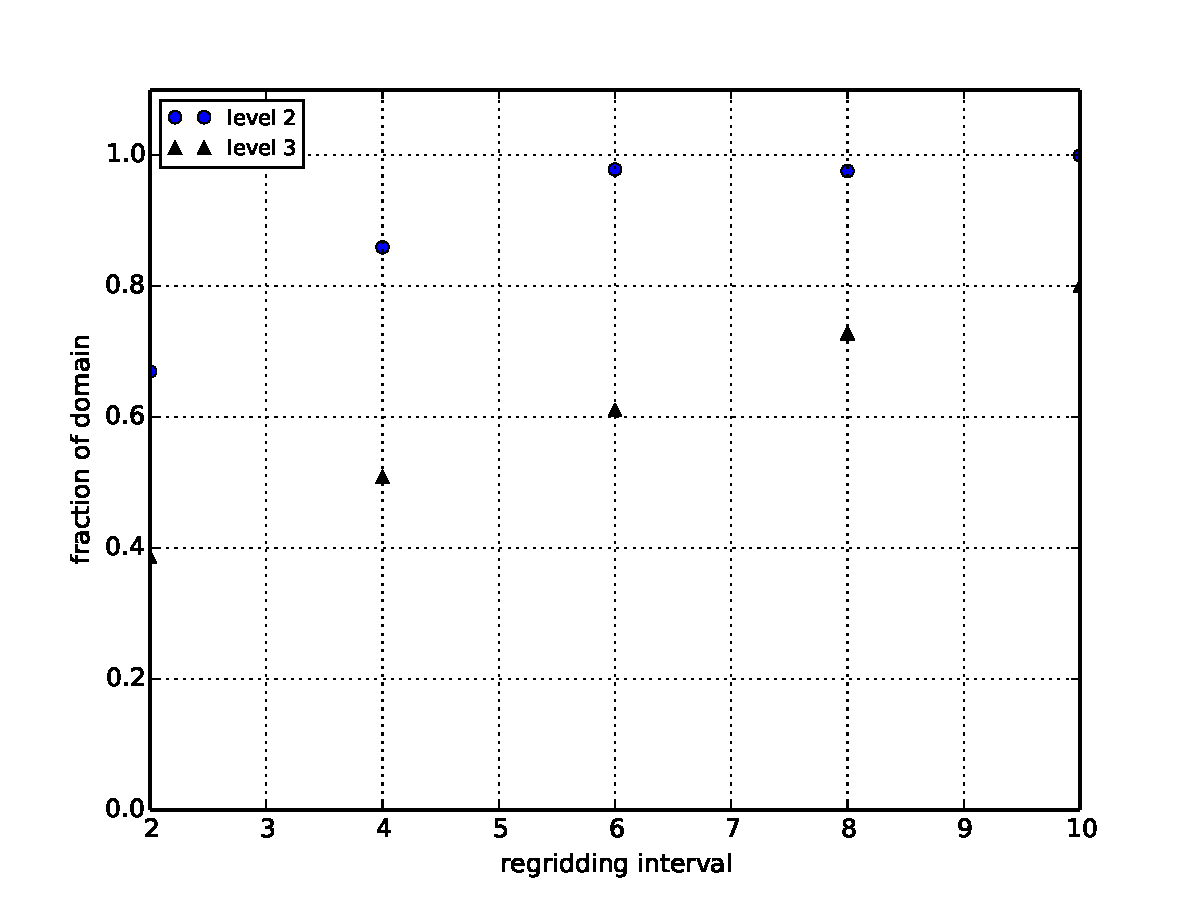
\includegraphics[width=0.85\textwidth]{myclaw/avg_cells_euler}
\label{fig:avg_cells_euler}
\end{figure}

\begin{figure}[!htb]
\centering
	\begin{subfigure}[b]{0.65\textwidth}
		\caption{Advection with interval/buffer~=~4}
		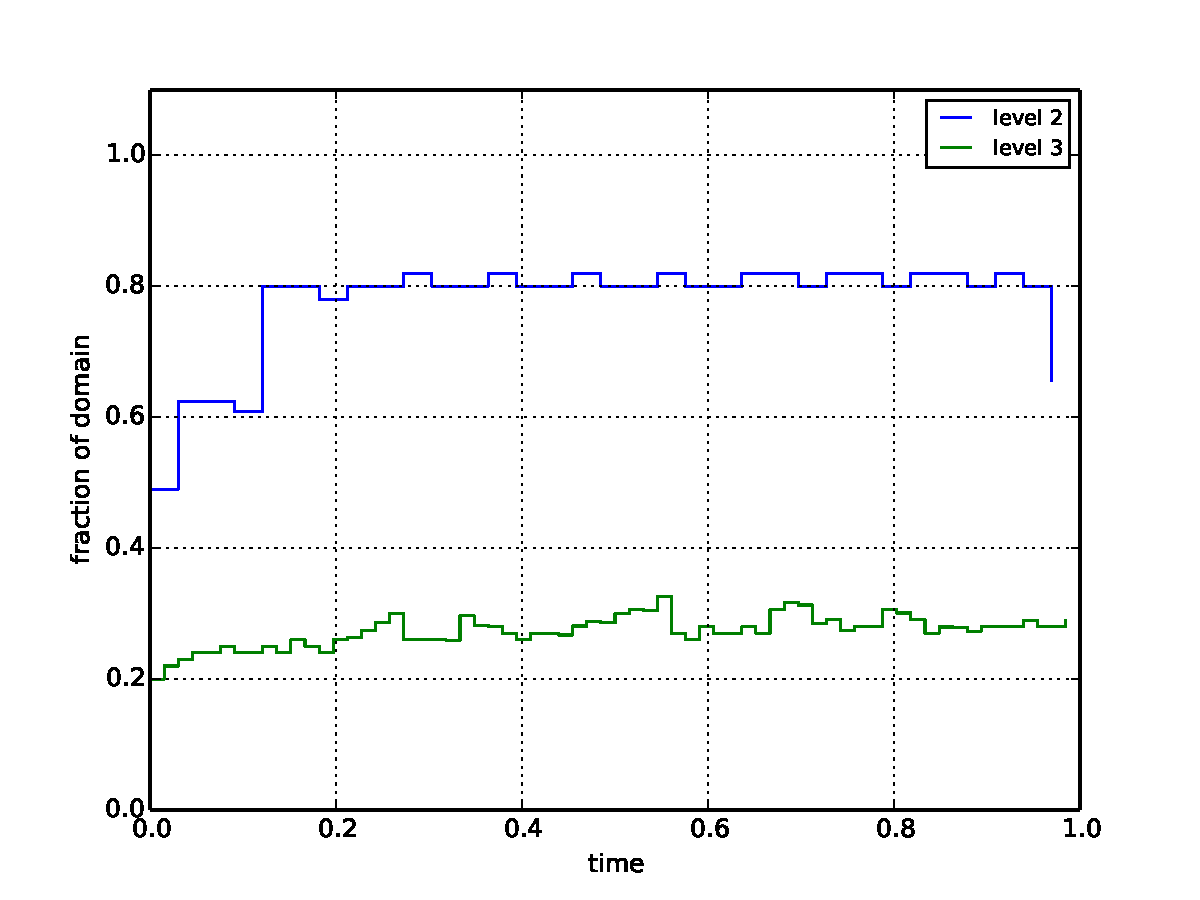
\includegraphics[width=\textwidth]{myclaw/cells_advec_4}
	\end{subfigure}
	
	\begin{subfigure}[b]{0.45\textwidth}
		\caption{Euler with interval/buffer~=~2}
		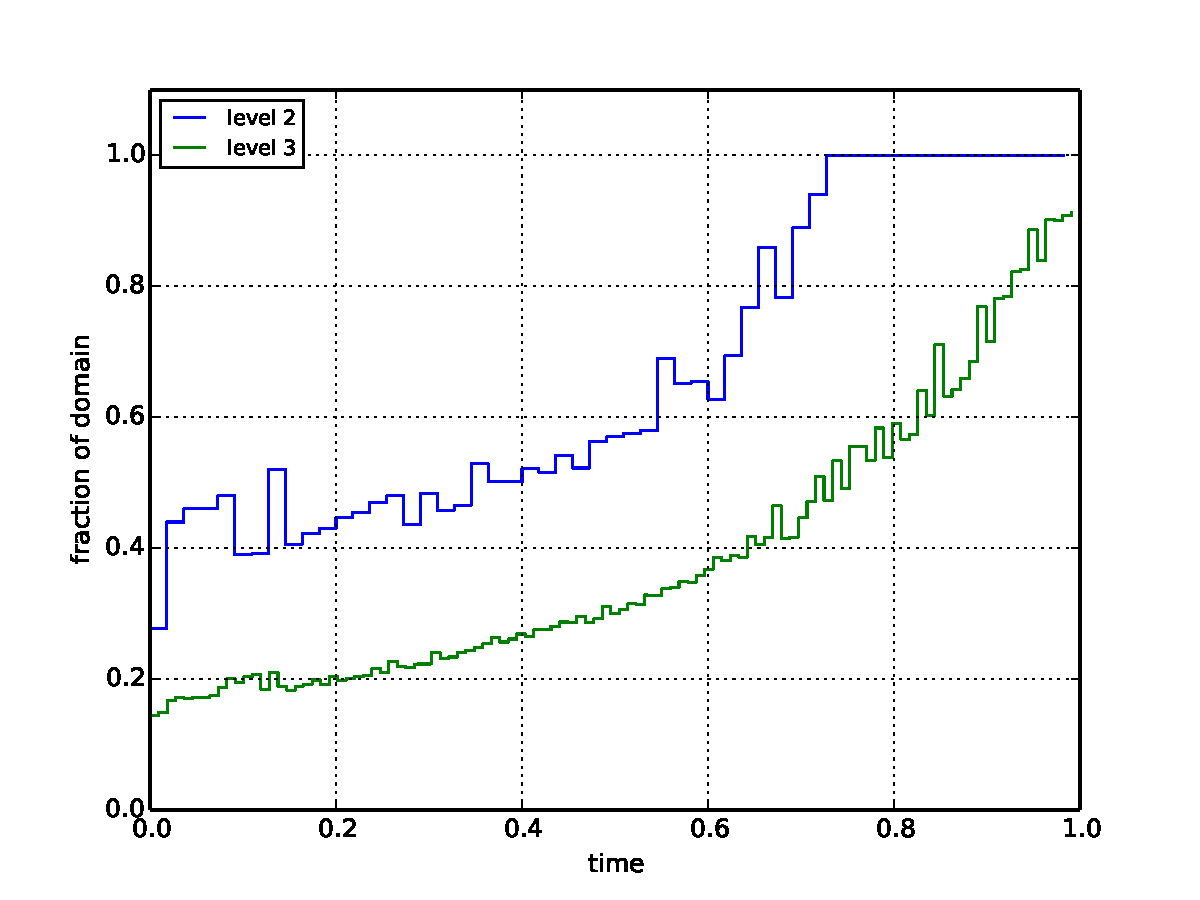
\includegraphics[width=\textwidth]{myclaw/cells_euler_2}
	\end{subfigure}	
	\begin{subfigure}[b]{0.45\textwidth}
		\caption{Euler with interval/buffer~=~8}
		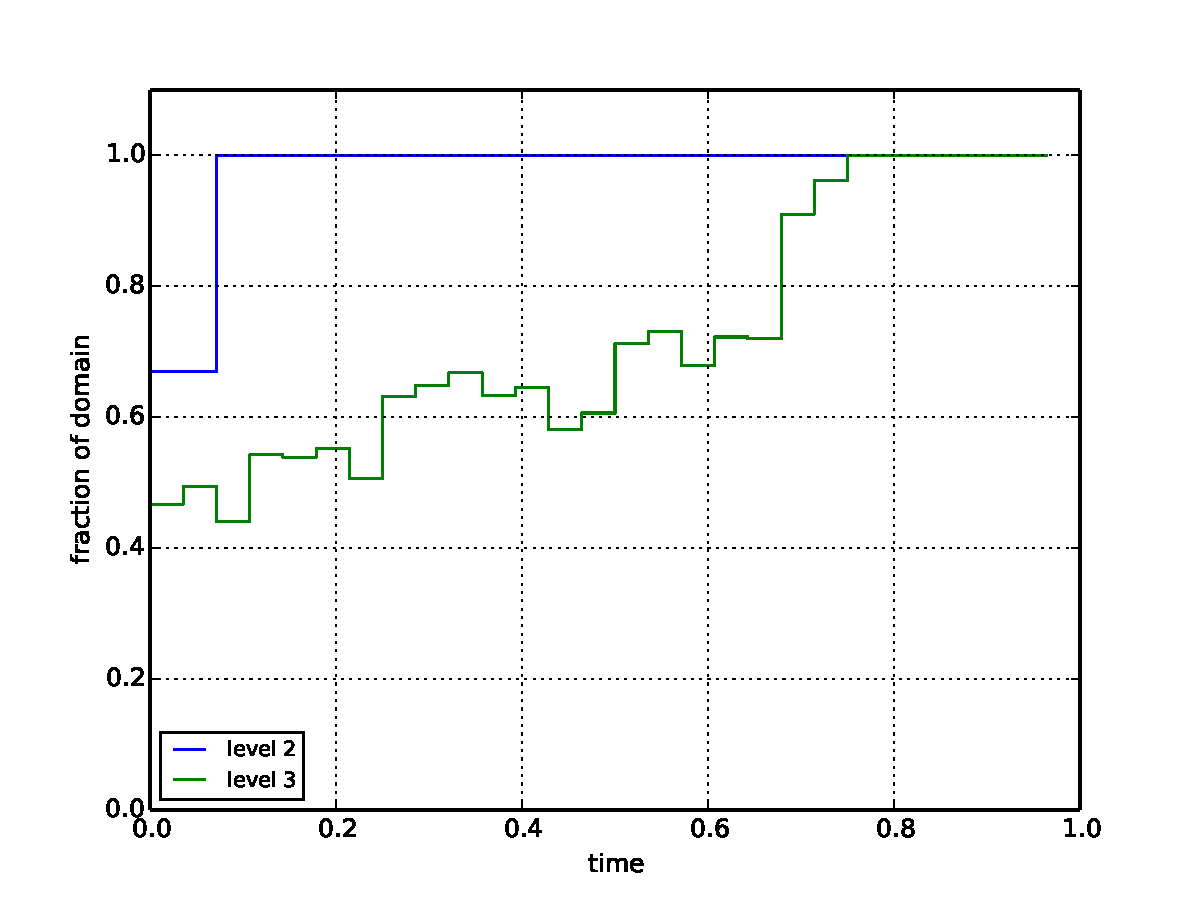
\includegraphics[width=\textwidth]{myclaw/cells_euler_8}
	\end{subfigure}
	\caption{A comparison of the number of cells over time (as a fraction
	of the total domain) for three different runs: advection with a medium
	interval/buffer, Euler with a small one, and Euler with a larger one}
	\label{fig:cells_over_time}
\end{figure}

\section*{Conclusions}
The relationship between the regridding interval and the buffer width
was clearly seen in both problems by the dramatic increase in error
when the regrid interval was allowed to increase without the buffer
following it. As was noted in the discussion of the Euler problem above,
this error introduced by having interesting features escape their
refined areas can manifest in qualitative impacts on the resulting
solution.

The trade-off between less time regridding but more time on finer
grid cells that a higher interval/buffer would bring proved to be
less interesting, with the grid time being dominant, and thus small
regrid intervals and the consequently smaller buffers they allow
seem unarguably preferable for these two problems. Indeed, the only
reason to avoid the absolute minimum of interval/buffer seems to be 
the (relatively) substantial drop in error that accompanies a shift to a slightly
higher interval/buffer (see Figures~\ref{fig:err_advec}~and~\ref{fig:err_euler}).

This relatively minor role for the regridding step does point in
the direction of possibly more sophisticated regridding setups 
(either in the criteria for refining, or the clustering or 
updating of cells) being a worthwhile pursuit, if they could offer
``smarter'' refinement that cuts down on finer meshes without
unduly increasing the error. Of course, it would need to be shown
that similar relationships around the regrid interval and buffer
width hold for problems of more interesting scale and complexity.

\section*{Ideas for Further Investigation}
As a starting point, it would be worthwhile to slightly modify the
parameter sweep and output parsing software to run multiple trials 
and aggregate the data; currently, the influence of random variation
in the running times is unknown. The general trends seem to follow 
expectation, but to be sure more data should be gathered. If I had more time,
I would have liked to use more gauges in computing the error in the solutions;
as it is currently I feel not enough data is actually being pulled from
the solutions to get an accurate picture of how close the solution is as
a whole.

More time to investigate would also allow for runs over more parameters, perhaps
of particular interest would be the number of levels and the refinement
ratios between them. It would interesting to see what differences (if any)
arise when comparing a set up that gradually refines over several levels
to one that has only a couple of levels but a more dramatic refinement
ratio. Simply running over wider ranges of existing parameters would
also be beneficial\footnote{However, larger domains would be needed to 
avoid filling in the whole space with the finest grids so quickly} by
giving a better sense of the rate at which running times and errors
change in response to the regridding interval and buffer.

It would also be interesting to explore more computationally intensive
regridding options, such as the Richardson extrapolation option provided
in AMRClaw (which estimates the difference between advancing on a finer grid
and the current grid, and flags cells where this difference exceeds a threshold;
this is the primary method mentioned in \cite{BergerLeVeque98}). A substantially
more time-consuming regridding step could make the trade-off between the
regrid interval and buffer width a more important consideration.

Problem-specific factors also no doubt play a large part in the interplay
between regridding intervals and buffers. For example, the advection of
the square produces regions of interest for refinement that align naturally
with the grid. This likely reduces the number of grids produced by allowing  
more efficient grouping of flagged points, but it also may increase the 
need for buffering those regions. Suppose instead the region being advected
were a diamond; the flagged regions would run diagonally, necessitating
grids that would naturally leave more buffer around many of the flagged points.
In contrast, for the square, the grid could cling much closer to flagged reasons,
leaving little buffer without explicitly requiring it. Similarly, the Euler 
quadrants problem has structures that seem to align diagonally to the grid,
and the opposite effects may arise if it were instead aligned 45$^o$ from its
present orientation.

Simply testing on a wider range of problems would be helpful to see which
elements of the regridding interval and buffer relationship are more generalizable.
In particular, in both the advection and Euler problems I examined, the areas of
interest formed a sizeable proportion of the total domain, leading to little
distinction between comfortably encompassing the interesting areas and simply
filling the entire domain with finer grids. Expanding the domain of the
two problems already examined would allow for a preliminary investigation into 
those issues.

\printbibliography


\end{document}